\subsection{Die Termistorkalibrierung}
Um den gemessenen Widerstand im Termistor einer Temperatur zuzuordnen, wird eine Kalibrierung durchgeführt. Hierzu wird der Termistor in das Kältebad gehalten. Die Temperatur des Kältebades wird wieder mit dem Digitalthermometer gemessen. Die Kalibrierung wird in einem Temperaturbereich von $-4^\circ C$ bis $2^\circ C$ durchgeführt. Der Widerstand wird alle $0.5^\circ C$ Differenz gemessen, während sich das Kältebad aufwärmt (im Fall dieser Versuchsreihe wurden zusätzlich einige Zwischenwerte dokumentiert).\\
Die Temperaturkurve des Termistors verhält sich exponentiell, allerdings ist für den entscheidenden Temperaturbereich im Bereich um die zwei Gefrierpunkte (welche in der Kalibrierung benutzt wird) eine lineare Näherung durchaus ausreichend. Die lineare Näherung\footnote{Berechnung durch Origin} besitzt eine Steigung $a$ und einen y-Achsenabschnitt $b$. Die Temperatur errechnet sich nun durch $a \cdot x + b$, wobei $x$ der Widerstand in $\unit[]{k\Omega}$ beschreibt. Folgende Werte ergeben sich bei der Annäherung an eine Gerade:

\begin{align*}
a &= \unit[(-3,215 \pm 0.024)]{\frac{K}{k\Omega}}\\
b &= \unit[(21,55 \pm 0.17)]{^\circ C}
\end{align*}
%
In diesen Fehlerwerten sind alle statistischen Fehler inbegriffen, sowohl die Fehlertoleranz des Thermometers als auch die Ungenauigkeiten bei der Messung und die durch die höhere Genauigkeit des Termistors (Mehrere Werte pro $\unit[0.1]{\Delta K}$) verursachten Schwankungen. Für die Messgeräte ist kein systematischer Fehler angegeben, also wird dieser als vernachlässigbar angenommen.


\begin{figure}
\begin{center}
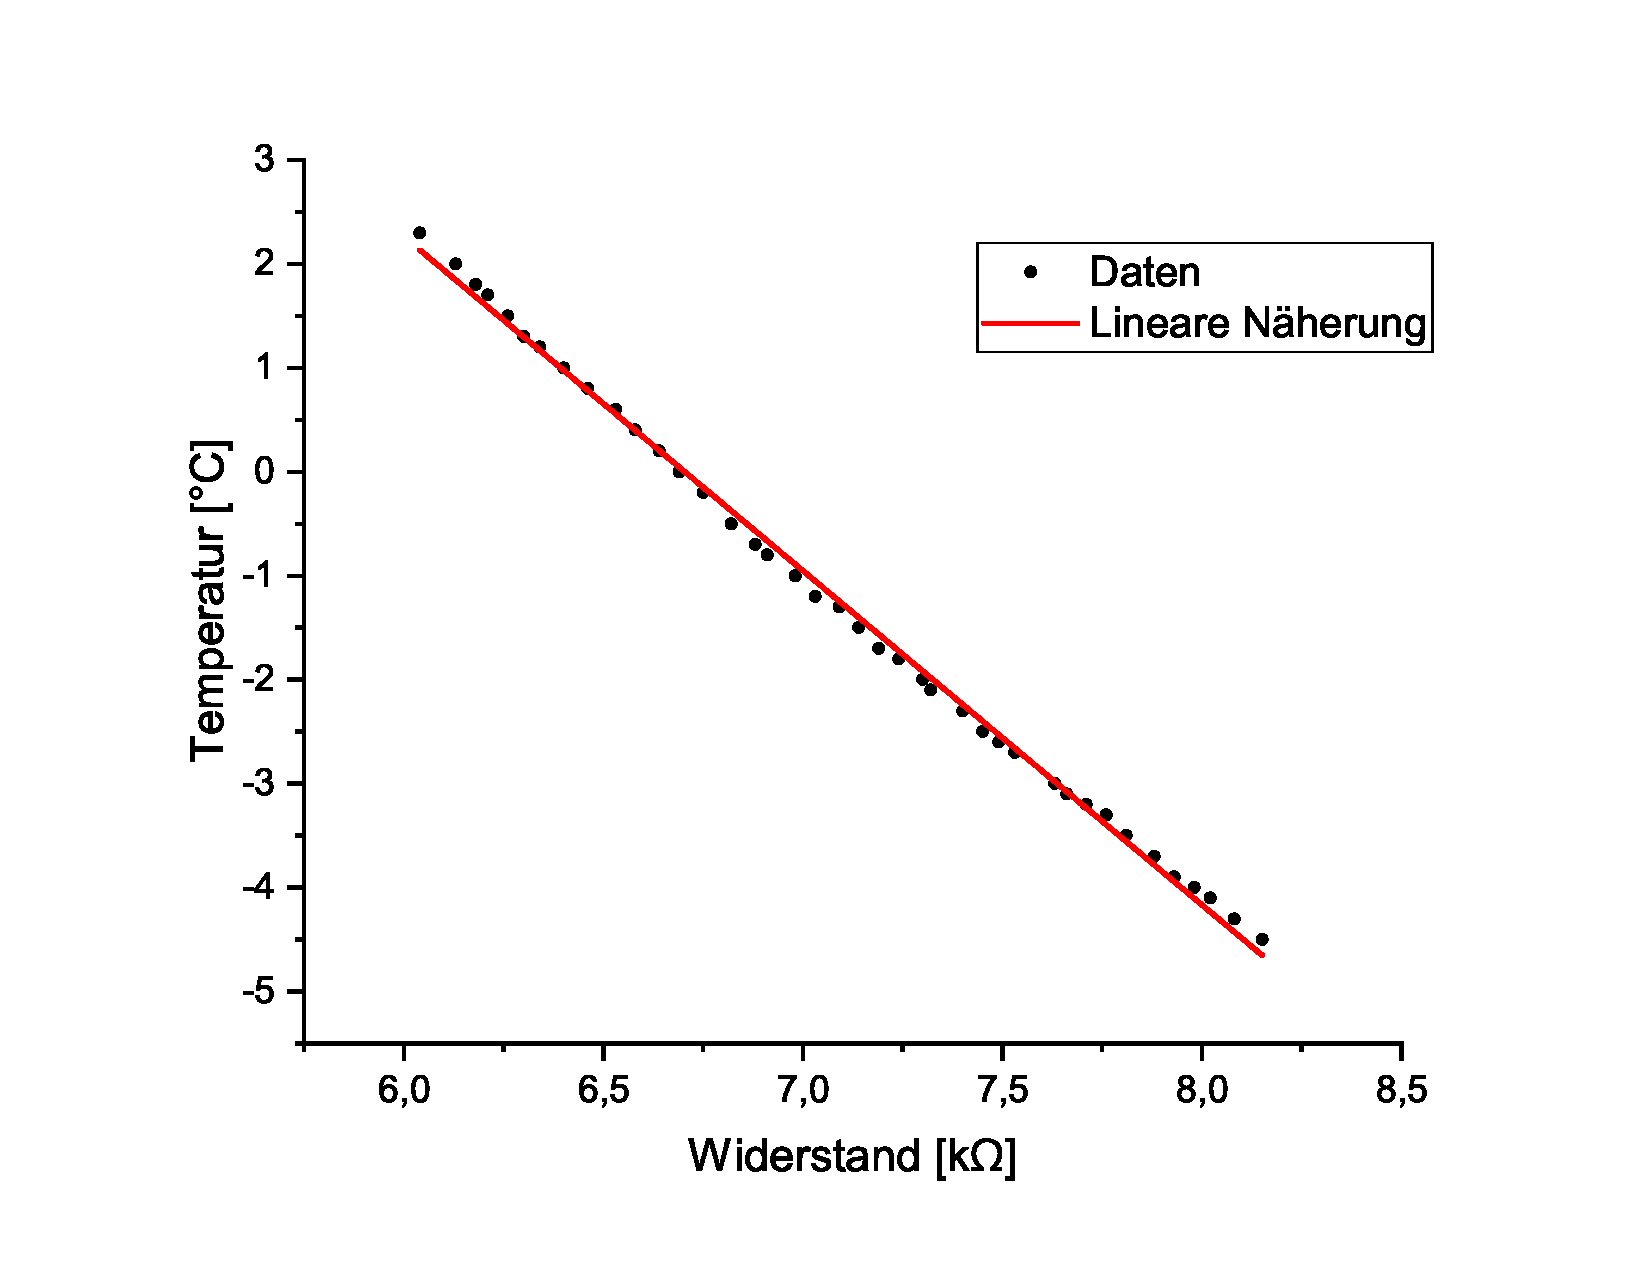
\includegraphics[scale=0.5]{Bilder/Kalibrierung_Termistor.eps}
\caption{Widerstand-Temperatur-Diagramm}
\end{center}
\end{figure}





